%=== CHAPTER FIVE ===
%% Implementation and experimental evaluation.  Rewritten 2026-09-18 against the
%% frozen SITL campaign of the deployed eventless interface.

\chapter{Implementation and Experimental Evaluation}
\label{ch:evaluation}
\begin{spacing}{1.5}
\setlength{\parskip}{0.22in}

\section{Software-in-the-Loop Platform}\label{sec:eval:platform}

The implementation is organised as ROS~2 packages around PX4
software-in-the-loop \cite{px4} and Gazebo \cite{gazebo}. The controller node
owns the reference generator, the predictive optimal control problem, the mission
sequence and the release-confirmation logic; the estimator node owns the sliding
measurement window, the physical-input reconstruction, the payload-state
optimisation, the lifecycle detector and the published payload frame. The two
communicate through the single atomic frame of
Section~\ref{sec:frame:interface}.

\begin{table}[ht]
\centering
\caption{Main implementation components of the deployed pipeline.}
\label{tab:software}
\small
\begin{tabularx}{\textwidth}{@{}l X X@{}}
\toprule
\textbf{Component} & \textbf{Role} & \textbf{Principal signals} \\
\midrule
Gazebo (Harmonic) & Rigid-body physics; detachable-joint gripper &
pose, rotor speed, attach/detach record (logging only) \\
PX4 SITL & State estimation, rate loop, control allocation &
odometry, actuator commands \\
\texttt{mhe\_node} & 16-state moving-horizon estimation; lifecycle detector &
odometry, rotor speed $\rightarrow$ payload frame \eqref{eq:frame} \\
\texttt{acados\_nmpc\_node} & Predictive control, mission sequence, confirmation &
payload frame, state $\rightarrow$ thrust and body-rate setpoint \\
\texttt{payload\_estimate} & Frame schema, confidence \eqref{eq:gamma}, release decision \eqref{eq:releasedecision} &
shared by the online node and the offline replay \\
\texttt{proximity\_gripper\_node} & Grasp contact and release actuation &
proximity, grasp enable, release command \\
\texttt{lifecycle\_trace} & Machine-readable event trace for scoring &
every state transition, with timestamps \\
\texttt{l1\_adaptive} & Comparison adaptive controller &
lumped matched disturbance $\bm d$, $\bm\xi$ \\
\texttt{px4\_pid\_benchmark} & Bare-autopilot cascade baseline &
position setpoints only \\
\bottomrule
\end{tabularx}
\end{table}

One platform decision is worth recording because it constrains what can be
claimed. Earlier work in this project used a Gazebo plugin that changed a link's
inertial properties at run time, which would have allowed a mass step without a
second body. That mechanism does not work: the simulator's component is written
and readable, but the physics engine continues to use the value from the model
description, so the vehicle never actually changes mass. Every payload change
reported here is therefore produced by the detachable-joint gripper, which
attaches and removes a genuine second rigid body and consequently couples mass,
inertia and centre of mass together. The retired mass-step line has been removed
from the repository, and no wrench-emulated result is retained.

\section{Platform Parameters}\label{sec:eval:params}

The reusable-vehicle constants are
\begin{equation}
\mB=\SI{2.0643}{\kg},\qquad
\Jb=\mathrm{diag}(0.0142,\,0.0142,\,0.0210)\ \si{\kg\meter\squared},\qquad
k_d=0.05 ,
\label{eq:platform}
\end{equation}
with rotor arm \SI{0.174}{\meter}, $k_f=\SI{8.55e-6}{\newton\second\squared}$ and
$k_m=\SI{0.016}{\meter}$. The collective-thrust box is the actuator envelope
\eqref{eq:envelope}, $[\SI{1.27}{\newton},\SI{31.35}{\newton}]$, and the torque
bounds are \SI{0.5}{\newton\meter} in roll and pitch and
\SI{0.2}{\newton\meter} in yaw. None of these grows with the estimate.

The value $\mB$ appears in the model, in the derived quantity
$\mP=(\mT-\mB)^{+}$ and in offline scoring. Payload masses of \SI{0.15}{\kg} and
\SI{0.30}{\kg} and grasp offsets up to \SI{0.15}{\meter} are used in the
experiments; none of these values is supplied to the estimator or the controller.

The task sequence is: approach under position control; hand-off to the predictive
controller and warm-up hover; controlled descent; grasp enable; lift;
figure-eight carry; phase-triggered release; recovery. The scope of the
controller is stated explicitly --- it governs the grasp hover and the
post-event adaptation phase, and the approach controller is not part of any
claim. Batches run headless.

\section{Experiment Design}\label{sec:eval:design}

The evaluation separates four questions: whether the payload states are
identifiable at all; whether the eventless interface completes a release; whether
refusing the command buys anything; and where the interface fails.

\subsection{Release-baseline arms}\label{sec:eval:arms}

The model-clearing logic is parameterised, so that the arms differ in exactly one
factor wherever possible. Table~\ref{tab:arms} lists them.

\begin{table}[ht]
\centering
\caption{Release baselines implemented as switchable arms. The estimator and the
controller each implement their half of the same named setting.}
\label{tab:arms}
\small
\begin{tabularx}{\textwidth}{@{}l l X@{}}
\toprule
\textbf{Arm} & \textbf{Name} & \textbf{Model-clearing rule} \\
\midrule
B & Eventless-Full & proposed: estimator evidence only; command never consulted \\
A & CMD-Immediate & clears payload geometry and inner-loop scaling at the release command, with no confirmation \\
C & CMD-Evidence & the proposed detector, but persistence counted only after the command arrives \\
--- & P-NoMoment & the proposed interface with the moment-gated path removed (mass domain only) \\
--- & Oracle & clears at the true separation instant; an upper bound, not deployable \\
\bottomrule
\end{tabularx}
\end{table}

Arm~A additionally uses the legacy, non-continuous geometry path and schedules
the inner loop by rewriting autopilot rate gains, whereas arm~B uses the
continuous frame and body-rate command scaling. The arms therefore differ
\emph{before} release as well as at it, and per-arm flight outcomes are reported
separately rather than pooled.

\subsection{Conditions and scenarios}\label{sec:eval:conditions}

Three nominal conditions are used: \SI{0.15}{\kg} at \SI{2}{\meter\per\second},
\SI{0.15}{\kg} at \SI{4}{\meter\per\second} and \SI{0.30}{\kg} at
\SI{4}{\meter\per\second}. The last is deliberately a stress test at the
vehicle's actuator limit rather than an operating point, for reasons quantified
in Section~\ref{sec:eval:limits}.

Five scenarios are run on top of those conditions:

\begin{enumerate}
\item \textbf{Nominal grasp--carry--release}, paired arm~A against arm~B.
\item \textbf{Delayed detachment.} A fault injector accepts the normal release
command but holds the physical joint for a median \SI{4.01}{\second}. This
separates ``the command was issued'' from ``the payload left''.
\item \textbf{Unsignaled loss.} The payload is detached at the release phase with
no command and no notification, emulating a gripper that opens by itself or a
load torn off.
\item \textbf{Partial loss.} Four \SI{0.05}{\kg} boxes are grasped together and
three are removed one at a time, at $45$, $80$ and \SI{115}{\second} after
grasp, with no signal; a control arm carries the same boxes without loss.
\item \textbf{Thrust-map mismatch.} The estimator's thrust coefficient alone is
scaled by \SI{\pm5}{\percent}, leaving the plant and the throttle inversion
untouched. This emulates a mis-calibrated $k_f$ on real hardware, which
Section~\ref{sec:eval:limits} identifies as the leading transfer risk.
\end{enumerate}

Eligibility is declared before scoring: a flight enters the release statistics if
the payload physically attached, according to the gripper's own attach record,
and the vehicle survived to the release command. This differs from the
pre-registered rule, which judged attachment from the estimator's mass evidence
and therefore silently excluded flights whose estimator failed to recognise an
attached payload --- exactly the cases most worth reporting. Both denominators
are given wherever they differ.

\section{Metrics}\label{sec:eval:metrics}

Position tracking is summarised by
\begin{equation}
\mathrm{RMSE}_p = \sqrt{\frac{1}{K}\sum_{k=1}^{K}\bigl\lVert\bm p_k - \bm p^{\mathrm{ref}}_k\bigr\rVert_2^2}.
\label{eq:rmse}
\end{equation}
Estimator metrics are the composite-mass error, the first-moment error against an
offline reconstruction of truth, the fraction of samples resting on a bound, and
the number of window re-anchorings. Lifecycle metrics are the completion rate,
the confirmation delay measured from the release command to the end of the
\SI{1.0}{\second} confidence hold, the confirmation path taken, and the count of
declarations occurring before any command or injected loss. Computational metrics
are the median and upper percentiles of the solve time for both optimisers.

Ground truth is used only in offline scoring. For the first moment, truth is
reconstructed after the fact as $\mP r_y$ from the simulator-measured grasp
offset; it never reaches the estimator, which runs with no horizontal attachment
geometry at all.

\section{Real-Time Performance}\label{sec:eval:timing}

On one desktop core shared with the simulator and the autopilot, the 13-state
controller ($N=20$, \SI{20}{\hertz}) solves in \SI{1.3}{\milli\second} at the
median and \SI{2.2}{\milli\second} at the 99th percentile over $n=1009$ solves:
\SI{2.6}{\percent} and \SI{4.4}{\percent} of its \SI{50}{\milli\second} period.

The 16-state estimator ($N=20$, \SI{10}{\hertz}) solves in
\SI{9.2}{\milli\second} at the median, \SI{24.6}{\milli\second} at the 90th and
\SI{59.2}{\milli\second} at the 99th percentile, with a \SI{72.8}{\milli\second}
maximum over $n=3740$ solves (the first twenty frames of each flight discarded),
against a \SI{100}{\milli\second} period. This is roughly seven times the
\SI{1.4}{\milli\second} median of the historical mass-only estimator: augmenting
the first moment costs no additional sensing, as Chapter~\ref{ch:model} argued,
but it is not computationally free.

The deadline is met in simulation and the tail margin is narrow. We therefore
make \emph{no} claim about headroom on an onboard computer; that requires
measurement on the target hardware.

\section{Estimation of the Payload States}\label{sec:eval:estimation}

Figure~\ref{fig:moment} shows the first-moment estimate against reconstructed
truth over eleven \SI{0.15}{\kg} flights at \SI{2}{\meter\per\second}. The
qualitative behaviour is the one the design intends: $\hat s_y$ is zero before
grasp, rises with no attach notification, holds near truth through the
figure-eight, and decays to zero after release rather than stepping.

\begin{figure}[ht]
\centering
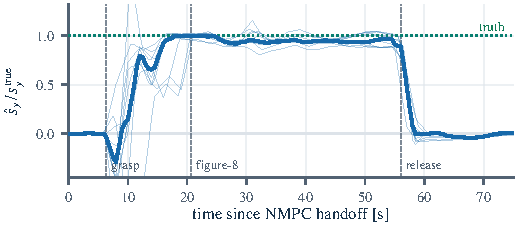
\includegraphics[width=0.92\textwidth]{Figures/fig_moment_truth.pdf}
\caption{First mass moment against ground truth (\SI{0.15}{\kg} at
\SI{2}{\meter\per\second}, $n=11$, each flight normalised by its own truth).
Truth is reconstructed offline from the simulator-measured grasp offset and never
reaches the estimator. The carry-phase estimate is biased toward zero in the
batch shown; the cause is not identified. The moment-gated detector uses the
ratio $\rho$ of \eqref{eq:rho}, which is insensitive to a common scale bias.}
\label{fig:moment}
\end{figure}

Two observations qualify the figure. First, the carry-phase estimate carries a
bias toward zero whose cause has not been identified; this is one reason the
detector is built on the ratio \eqref{eq:rho} rather than on an absolute
magnitude, since a common scale factor cancels in the ratio. Second, the $s_x$
(pitch) channel is consistently noisier than the $s_y$ (roll) channel, which
matches the torque-reconstruction correlations reported in
Section~\ref{sec:model:phys}.

Figure~\ref{fig:track3d} shows two complete missions in three dimensions,
including the two distinct post-release behaviours that
Section~\ref{sec:eval:completion} quantifies.

\begin{figure}[ht]
\centering
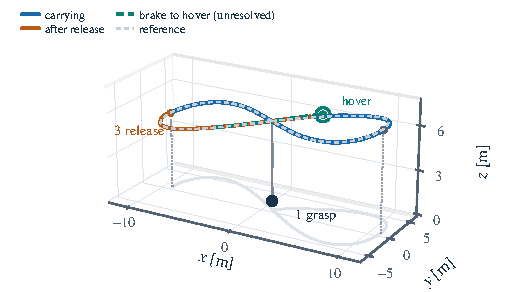
\includegraphics[width=0.92\textwidth]{Figures/fig_track_3d_measured.pdf}
\caption{Measured mission trajectory (simulator ground truth), two
\SI{0.15}{\kg}/\SI{2}{\meter\per\second} flights of the same batch: grasp, lift,
then carry along the figure-eight with \SI{\pm0.8}{\meter} vertical undulation
against the nominal reference. After the release command one flight clears the
moment vote in manoeuvre and keeps tracking; the other declares
\textsc{unresolved} at its \SI{12}{\second} timeout and brakes to hover,
confirming at \SI{16.40}{\second}. The two paths agree to within
\SI{0.12}{\meter} (median) before the timeout. Loaded tracking RMS is
\SI{0.053}{\meter} and \SI{0.060}{\meter} after release.}
\label{fig:track3d}
\end{figure}

\section{Completion and Confirmation Delay}\label{sec:eval:completion}

The complete interface confirmed release in 32 of 36 eligible flights
(Table~\ref{tab:complete}); the two-sided \SI{95}{\percent} Clopper--Pearson
interval is $[\SI{73.9}{\percent},\SI{96.9}{\percent}]$. All four failures
occurred at \SI{4}{\meter\per\second} and all four trace to estimator failure
rather than to the decision logic: three never recognised the payload and
remained \textsc{unresolved}, and one diverged after release. The pre-registered
eligibility rule would have excluded the first three and reported $31/32$; the
rule adopted here retains them.

\begin{table}[ht]
\centering
\caption{Release completion and confirmation delay, all eligible arm~B flights.
Delay runs from the release command to the end of the \SI{1.0}{\second}
confidence hold and is computed over completed flights. The two delay columns are
distinct control paths and are not pooled.}
\label{tab:complete}
\small
\begin{tabular}{@{}lcccc@{}}
\toprule
 & & & \multicolumn{2}{c}{delay median [IQR]} \\
\cmidrule(lr){4-5}
condition & $n$ & compl. & in manoeuvre & via brake-to-hover \\
\midrule
\SI{0.15}{\kg}, \SI{4}{\meter\per\second} & 11 & 10/11 & \SI{2.90}{\second} [2.90, 2.90] & \SI{16.60}{\second} [16.60, 16.60] \\
\SI{0.30}{\kg}, \SI{4}{\meter\per\second} & 13 & 10/13 & \SI{8.95}{\second} [8.00, 9.26] & \SI{16.40}{\second} [16.20, 16.70] \\
\SI{0.15}{\kg}, \SI{2}{\meter\per\second} & 12 & 12/12 & \SI{3.31}{\second} [2.95, 4.36] & \SI{16.48}{\second} [16.40, 16.50] \\
\midrule
pooled & 36 & 32/36 & \SI{3.46}{\second} [2.90, 8.00] & \SI{16.56}{\second} [16.46, 16.60] \\
\bottomrule
\end{tabular}
\\[4pt]
\footnotesize Overall delay maximum \SI{16.70}{\second}. Share confirming only
after braking to hover: \SI{50}{\percent}, \SI{40}{\percent},
\SI{50}{\percent} of completed flights by row, \SI{47}{\percent} pooled.
\end{table}

The confirmation delay is \emph{bimodal}, and the two modes correspond to the two
paths of Section~\ref{sec:frame:unresolved} rather than to a spread within one
mechanism. In 17 of the 32 completed flights the confidence crosses its threshold
while the vehicle is still flying the figure-eight, and confirmation completes in
a median of \SI{3.46}{\second}. In the remaining 15, no release evidence is
available in manoeuvre --- either $\hat\svec$ has drifted under sustained
excitation, or the frozen reference of Section~\ref{sec:frame:momentref} never
formed --- so the system reaches its \SI{12}{\second} timeout, declares
\textsc{unresolved}, brakes to hover over \SI{3}{\second}, and confirms at a
median of \SI{16.56}{\second}. Pooling the two would describe neither.

Figure~\ref{fig:mission} shows one complete in-manoeuvre confirmation.

\begin{figure}[ht]
\centering
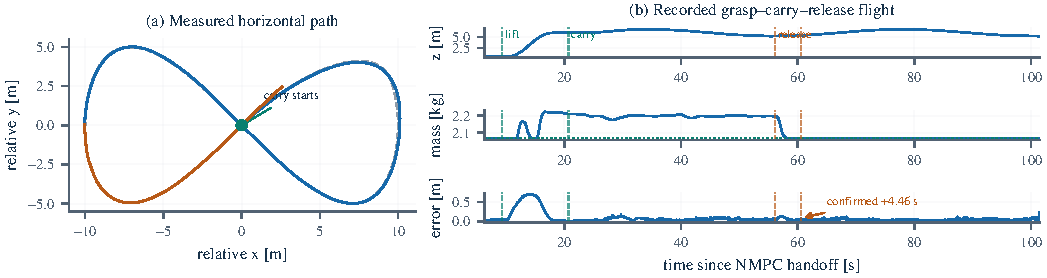
\includegraphics[width=0.96\textwidth]{Figures/fig_mission.pdf}
\caption{One eventless flight from the final batch (\SI{0.15}{\kg},
\SI{2}{\meter\per\second}). Left: measured horizontal path, coloured by carrying
and post-release phase, against the nominal reference including its amplitude
ramp. Right: height, the mass estimate actually consumed by the controller, and
the position-error norm through grasp, lift, carry, release command and
confirmation. This flight confirms in manoeuvre \SI{4.46}{\second} after the
command; it illustrates one execution and does not replace the cohort statistics
of Table~\ref{tab:complete}.}
\label{fig:mission}
\end{figure}

Table~\ref{tab:paths} records which route produced each confirmation. Every
confirmation used the controller's confidence route \eqref{eq:confirm}; the
columns record the estimator declaration, where one occurred. That three distinct
routes appear is the reason the completion rate must be read as a result for the
\emph{interface as a whole} rather than as a validation of any single detector.

\begin{table}[ht]
\centering
\caption{Confirmation paths in the 32 completed flights of
Table~\ref{tab:complete}. \emph{Moment-gated}: the detector declared before the
confidence crossed. \emph{Mass-domain}: the frozen reference never formed, the
confidence crossed during or shortly after the brake to hover, and the
mass-domain route declared \SIrange{0.9}{3.1}{\second} later. \emph{Confidence
only}: the reference never formed and no declaration occurred.}
\label{tab:paths}
\small
\begin{tabular}{@{}lcccc@{}}
\toprule
condition & $n$ & moment-gated & mass-domain & confidence only \\
\midrule
\SI{0.15}{\kg}, \SI{4}{\meter\per\second} & 10 & 9 & 1 & 0 \\
\SI{0.30}{\kg}, \SI{4}{\meter\per\second} & 10 & 1 & 3 & 6 \\
\SI{0.15}{\kg}, \SI{2}{\meter\per\second} & 12 & 9 & 0 & 3 \\
\midrule
pooled & 32 & 19 & 4 & 9 \\
\bottomrule
\end{tabular}
\end{table}

No flight in any path declared release before the command. In 23 of the 32
completed flights the presence machine made exactly two transitions, one at grasp
and one at release; in the nine confidence-only flights it never declared
\textsc{empty} within the logged window, which extended more than
\SI{40}{\second} past confirmation. Every load declaration came from sustained
mass evidence, and no external grasp signal was consumed.

\section{Does Refusing the Command Buy Anything?}\label{sec:eval:paired}

\subsection{Nominal pairs}\label{sec:eval:nominal}

Across 19 pairs in which both arms were eligible, both arms completed $19/19$
releases with no observed post-release instability
(Table~\ref{tab:paired-event}). Arm~A has zero confirmation delay by
construction. Under nominal conditions, therefore, refusing the command buys
nothing and costs a delay --- which is the correct result, since nominal
conditions are precisely those in which the command is true.

\begin{table}[ht]
\centering
\caption{Paired command-triggered ablation. Arm~A clears the model at the command
by construction; arm~B requires estimator evidence; arm~C is arm~B with its
release evidence armed only by the command. The last two rows inject a
command/physical-detachment mismatch; ``early'' means model clearing before the
joint is actually removed (``--'': not scored).}
\label{tab:paired-event}
\small
\begin{tabular}{@{}lcccc@{}}
\toprule
condition & pairs & A compl. & B compl. & early clear A/B \\
\midrule
\SI{0.15}{\kg}, \SI{4}{\meter\per\second} & 8 & 8/8 & 8/8 & -- \\
\SI{0.30}{\kg}, \SI{4}{\meter\per\second} & 3 & 3/3 & 3/3 & -- \\
\SI{0.15}{\kg}, \SI{2}{\meter\per\second} & 8 & 8/8 & 8/8 & -- \\
\midrule
nominal pooled & 19 & 19/19 & 19/19 & -- \\
\SI{0.15}{\kg}, \SI{2}{\meter\per\second} $+$ \SI{4}{\second} hold & 5 & 5/5 & 5/5 & 5/5 \ / \ 0/5 \\
\quad same, arm~C instead of A & 6 & 6/6 (C) & 6/6 & 0/6 \ / \ 0/6 \\
\bottomrule
\end{tabular}
\end{table}

Only three pairs formed at the \SI{0.30}{\kg}/\SI{4}{\meter\per\second}
condition, because arm~A crashed during or immediately after lift in 11 of 16
attempts there. That failure is a property of arm~A's gain-rewriting schedule
rather than of its release semantics: its rate scaling starts from the
lower-bound mass estimate while the box is still resting on the ground.

\subsection{Delayed detachment}\label{sec:eval:delayed}

Under a median \SI{4.01}{\second} hold between command and physical detachment,
the arms separate exactly as designed. Of twelve arm-runs one arm~A run never
armed the autopilot, leaving five valid pairs and one valid unpaired arm~B run.

In all five pairs arm~A cleared its payload model at the command, a median
\SI{4.01}{\second} before the payload actually left. Arm~B cleared before
detachment in \emph{none} of its six valid runs: it entered \textsc{unresolved}
in $5/6$ and confirmed a median \SI{12.45}{\second} after detachment, while the
remaining run confirmed \SI{3.00}{\second} after detachment. All eleven valid
runs carried an independent simulator detachment record.

The honest reading of this result is narrow. Median position-error peaks during
the hold were \SI{0.071}{\meter} for arm~A and \SI{0.068}{\meter} for arm~B, so
what the experiment demonstrates is a difference in \emph{model--plant
consistency}, not a tracking advantage and not crash avoidance. A permanently
jammed gripper --- under which arm~A would fly a loaded vehicle with an empty
model for the remainder of the mission --- was not tested.

\subsection{Command-armed confirmation and unsignaled loss}\label{sec:eval:unsignaled}

The delayed-detachment result reflects \emph{persistent confirmation}, not
eventlessness. Arm~C demonstrates this directly: armed only by the command but
otherwise identical to arm~B, it also never cleared early ($0/6$ pairs) and
confirmed sooner after detachment (median \SI{4.3}{\second} against
\SI{7.3}{\second}). If the only hazard were a slow gripper, arm~C would be the
better design.

Eventlessness earns its keep when no release command reaches the controller at
all. With such losses injected at the release phase, arm~B detected the loss in
10 of 18 paired flights --- $4/9$ at \SI{2}{\meter\per\second}, and $4/5$ and
$2/4$ at \SI{0.15}{\kg} and \SI{0.30}{\kg} at \SI{4}{\meter\per\second}, with a
median latency of \SIrange{2.2}{2.9}{\second} --- while arm~C, never armed,
detected none and carried a phantom first moment for the rest of the flight.
Seven of the eight misses occurred because the loaded moment reference had not
formed, or the payload had not been recognised, before the loss: the same
mechanism that produces the brake-to-hover mode in
Table~\ref{tab:complete}.

The cost of running a release detector throughout loaded flight --- the risk of a
false positive while the payload is still attached --- was measured and not
observed. No release was declared before a command or an injected loss in 209
loaded flights spanning \SI{3.7}{\hour}, giving a per-flight \SI{95}{\percent}
upper bound of \SI{1.4}{\percent}.

\section{Partial Payload Loss}\label{sec:eval:partial}

Losing part of a load is the case that a binary attached/detached abstraction
cannot represent at all, and it is where a continuous interface should show an
advantage in kind rather than in degree.

Pre-registered criteria were: (a) $\hat m$ enters $\pm\SI{0.02}{\kg}$ of each new
truth in at least \SI{80}{\percent} of steps; (b) the paired tracking-RMS
difference against the no-loss control arm is at most \SI{0.02}{\meter}, with no
crash; (c) no \textsc{empty} declaration after the first two losses.

At \SI{2}{\meter\per\second} all three criteria pass: the estimate followed 14 of
15 steps, with a median convergence of \SIrange{1.1}{8.8}{\second}, there was no
false \textsc{empty} declaration, and tracking was indistinguishable from the
control arm. At \SI{4}{\meter\per\second} criterion (a) reached only its
threshold ($12/15$), so recovery is claimed at \SI{2}{\meter\per\second} only.

\section{Ablations}\label{sec:eval:ablations}

\subsection{Thrust-map calibration}\label{sec:eval:thrustcal}

Section~\ref{sec:model:conline} predicted an asymmetry: the centre-of-mass
inversion is immune to the thrust coefficient because $k_f$ cancels
\eqref{eq:kfcancel}, whereas the mass channel consumes an absolute thrust and
therefore inherits the calibration error directly. The experiment confirms it,
and the sensitivity is severe.

Scaling only the estimator's thrust map by \SI{\pm5}{\percent}
(\SI{0.15}{\kg}, \SI{2}{\meter\per\second}, four repetitions per arm, 11 valid
flights) caused no pre-command release in any arm, but defeated the interface in
both directions:
\begin{itemize}
\item at $0.95$, the payload was never recognised ($0/3$) and every flight
remained \textsc{unresolved};
\item at $1.05$, a phantom \SI{+0.09}{\kg} persisted after release ($4/4$), every
flight remained \textsc{unresolved}, and one diverged;
\item at the matched value $1.00$, the payload was recognised in $4/4$.
\end{itemize}

The interpretation is that $k_f$ must be calibrated well inside \SI{5}{\percent}
for this interface to function. That is a demanding requirement, and it is the
single most important item for hardware transfer. Note also what the failure mode
is: not a wrong release, but a refusal to confirm. The interface degrades toward
\textsc{unresolved} rather than toward an empty model, which is the correct
direction for a safety-relevant decision, but it is still a failure.

\subsection{Window-balance re-initialisation}\label{sec:eval:seed}

The window vertical-force seed of \eqref{eq:winbal} replaced the instantaneous
hover approximation \eqref{eq:massseed}. A pre-registered A/B comparison at the
\SI{4}{\meter\per\second} condition gives: valid flights $10/10$ with the window
seed against $8/10$ without; figure-eight re-initialisations reduced from 29 to
1; seed error reduced from \SI{17.1}{\percent} to \SI{2.8}{\percent}; longest
consecutive re-initialisation run reduced from 17 to 1; mission completion
$10/10$ with no post-release crash.

One reservation is recorded with the result: in the enabled arm only a single
re-initialisation event occurred, so the mechanism was barely exercised there.
The reported lifecycle cohort predates this change.

\subsection{The inertia-coefficient mode}\label{sec:eval:amode}

The three alternatives to \eqref{eq:Afrozen} behave as the analysis of
Section~\ref{sec:model:Amode} predicts. In synthetic grasp--release replay, the
\textsf{coupled} mode drives the post-release mass estimate up by
\SI{53}{\percent} and holds it there; the \textsf{frozen} mode returns to
\SI{-0.34}{\percent} of the bare airframe with $\svec$ and $\dJ$ decaying
together and no bound contact. In closed loop, the \textsf{const} mode --- which
also removes the derivative, but pins the coefficient to the payload envelope ---
biases the loaded mass estimate to \SI{-3.58}{\percent} against \SI{+0.4}{\percent}
for \textsf{frozen}, and that bias was sufficient to make the mass-domain release
criterion fire prematurely, \SI{50}{\second} before the true detachment. Fixing
the derivative is necessary; fixing the \emph{value} is harmful.

\subsection{A negative result on learned stage weights}\label{sec:eval:weightlearning}

The parameterised generalisation of the retired event-triggered schedule
(Section~\ref{sec:frame:beta}) was optimised by cross-entropy search in the loop,
and the resulting schedule showed no measurable benefit over the hand-designed
rule in a paired ablation. The objective was flat over a broad neighbourhood of
that rule.

This negative result is substantively useful, and is reported rather than
omitted. What produced the benefit in the predecessor system was \emph{noticing
that the model had changed and removing stale data}; the precise magnitude of the
post-trigger weights is weakly determined by the data. A learned schedule should
therefore not be presented as a superior learned controller. It is also part of
the reason the mainline retired event logic altogether.

\section{Where the Interface Fails}\label{sec:eval:limits}

\subsection{Moment-reference formation}\label{sec:eval:refform}

The dominant failure mode is not a wrong decision but an unavailable one. In 13
of the 32 completed flights the healthy, low-dynamic, in-envelope window of
Section~\ref{sec:frame:momentref} never filled after the \textsc{loaded}
declaration, so the ratio test never ran at all. Those flights are the population
of the brake-to-hover column of Table~\ref{tab:complete} and of seven of the
eight unsignaled-loss misses.

A contributing factor was found and is smaller than the effect: the
admissibility envelope \eqref{eq:sadmissible} assumed a \SI{0.13}{\meter} grasp
offset while the gripper actually admitted \SI{0.15}{\meter}, which affected 2 of
13 \SI{0.30}{\kg} flights. It does not explain most of the missing references.
Reliable reference formation therefore remains necessary work.

A related boundary is recorded honestly: out-of-envelope $\hat\svec$ samples are
excluded from moment votes but still reach the controller's $\cvec$ through the
filter and slew limiter of \eqref{eq:lpfslew}. The exclusion protects the
decision, not the model.

\subsection{First-moment drift under sustained excitation}\label{sec:eval:drift}

Sustained figure-eight excitation can raise $\lVert\hat\svec\rVert$ from
\SI{0.012}{\kg\meter} to \SI{0.031}{\kg\meter}. Because moment evidence is then
withheld, confirmation is delayed. Deceleration restored the vote within
\SIrange{3.3}{3.4}{\second} in the affected flights, which is the mechanism
behind the brake-to-hover delays.

An online counter of envelope exceedances correlates with this outcome at
\SI{4}{\meter\per\second} --- in-manoeuvre confirmation occurred in $9/10$
flights with zero exceedances against $2/10$ otherwise, Fisher exact
$p=0.006$ --- but it misses all six delayed \SI{2}{\meter\per\second} cases, so it
is a partial diagnostic rather than a predictor. Exiting the manoeuvre earlier on
that signal is unimplemented and unvalidated.

\subsection{The operating limit}\label{sec:eval:opslimit}

\SI{0.30}{\kg} at \SI{4}{\meter\per\second} is at the vehicle's actuator limit.
Hover requires \SI{74}{\percent} of maximum thrust, but it is torque, not thrust,
that binds: in the figure-eight, pitch torque saturated within \SI{98}{\percent}
of five-second diagnostic windows and yaw within \SI{53}{\percent}
(\SI{46}{\percent} and \SI{16}{\percent} at \SI{0.15}{\kg}, at most
\SI{6}{\percent} at \SI{2}{\meter\per\second}), and the body-rate scaling of
\eqref{eq:omegascale} ran at a median $4.39$ of its cap of $5.0$. This is the
quantitative form of the feasibility boundary predicted by \eqref{eq:trimtorque}
and \eqref{eq:gain} in Chapter~\ref{ch:model}.

Three of the five arm~B pre-release crashes and three of the four incomplete
releases occurred at this condition. Every eligible \SI{2}{\meter\per\second}
flight confirmed its release. What is claimed at this limit is safe release
\emph{semantics}, not reliable flight; deployment there needs torque margin.

\subsection{Estimator failures}\label{sec:eval:estfail}

In four flights the published mass never left the empty value; in two of these,
repeated solver failures caused re-initialisation from a lower-bound seed. The
three at \SI{4}{\meter\per\second} flew without diverging and remained
\textsc{unresolved}.

One failure is more instructive than the rest. In a \SI{0.30}{\kg} flight the
estimate was unhealthy for \SI{48}{\second} before release. Because the
phase-timed release command is \emph{not} gated on estimator health, the command
was issued anyway; the frozen model no longer matched the vehicle after
detachment, and the flight diverged. Gating release on estimator health is an
obvious remedy and is not implemented.

\subsection{Configuration and default-safety}\label{sec:eval:defaults}

Every reported release batch explicitly enables the release-evidence path. Its
built-in default is \emph{off}, under which every flight ends
\textsc{unresolved}. Deployment therefore requires an explicit enable plus
startup validation of the configuration, and the implementation includes a
self-check that reports at startup which blockers, if any, would prevent the
detector from ever firing.

\subsection{Missing baselines}\label{sec:eval:missing}

The only baselines reported here are the command-triggered and command-armed arms
of Table~\ref{tab:arms}, which isolate release semantics. The evaluation does
\emph{not} include a comparison against a fixed-parameter predictive controller,
against a lumped-disturbance adaptive method such as $\mathcal{L}_1$-adaptive
NMPC \cite{hanover2021} or incremental nonlinear dynamic inversion
\cite{smeur}, or against a change-detection procedure such as CUSUM
\cite{basseville1993} applied to the same signals under a matched false-alarm
constraint. Comparison nodes for the first two exist in the implementation
(Table~\ref{tab:software}) but no frozen result set is reported for them. This is
the largest gap in the evaluation and is stated as such.

\section{Threats to Validity and Reproducibility}\label{sec:eval:validity}

All system-level evidence is software-in-the-loop. The leading threats are:

\begin{itemize}
\item \textbf{Thrust-map fidelity.} The plant generates thrust with the same
square law the estimator inverts, and rotor speeds are exact. The
\SI{\pm5}{\percent} experiment of Section~\ref{sec:eval:thrustcal} bounds one
dimension of this; speed noise, transport delay and induced inflow
\cite{bangura2012} remain untested.
\item \textbf{Clean state estimates.} The odometry available in simulation is
better than a real vehicle's, and the measurement weights \eqref{eq:Wy} are set
from representative rather than measured noise levels.
\item \textbf{Rigid attachment.} Gripper compliance and pendulum modes are not
modelled. Neither affects which signals the estimator consumes, but both would
add unmodelled dynamics to the rotational residual on which $\svec$ depends.
\item \textbf{Confounded disturbances.} A sustained vertical updraft or downdraft
is intrinsically indistinguishable from a payload change on a
collective-thrust-only residual. Wind is not evaluated in the reported cohort.
\end{itemize}

Reproducibility is handled by construction rather than by discipline. Every run
records the software revision, the resolved value of every environment switch
that affects behaviour, the problem dimensions, horizons, weights, bounds, event
timestamps, random seed and solver statistics. Runs terminated by numerical
failure remain in the denominator. The release decision used online and the one
used in offline replay are the same function, so a recorded flight can be
re-scored without re-implementing the logic.

\begin{table}[ht]
\centering
\caption{Attempts and exclusions in the paired campaign. Because the arms differ
before release, these rates are reported per arm rather than pooled, and neither
characterises end-to-end mission reliability.}
\label{tab:attempts}
\small
\begin{tabularx}{\textwidth}{@{}l c X@{}}
\toprule
\textbf{Arm} & \textbf{Attempts} & \textbf{Disposition} \\
\midrule
B (proposed) & 42 & 36 eligible; 5 crashed before the release command (three in
the \SI{0.30}{\kg}/\SI{4}{\meter\per\second} figure-eight, two during lift at
\SI{2}{\meter\per\second}); 1 did not physically attach \\
A (command-triggered) & 42 & 25 eligible; 17 pre-release crashes, 11 of them
during or just after lift at \SI{0.30}{\kg}/\SI{4}{\meter\per\second} \\
\bottomrule
\end{tabularx}
\\[4pt]
\footnotesize Table~\ref{tab:paired-event} uses the 19 pairs with both arms
eligible; Table~\ref{tab:complete} uses all 36 eligible arm~B flights; and
Table~\ref{tab:paths} uses the 32 that completed. Tail-window tracking is not
compared, because arm~B brakes to hover after an unresolved timeout while arm~A
continues the figure-eight.
\end{table}

\section{Development-Stage Evidence}\label{sec:eval:devstage}

Two earlier tests motivated the final design but used earlier code and do not
validate the deployed detector. They are reported because the design decisions
they produced are load-bearing in Chapter~\ref{ch:framework}.

First, the quantity--residual fast branch without moment evidence declared release
prematurely in 3 of 9 randomised flights during a \SI{4}{\meter\per\second}
figure-eight, the earliest \SI{51.1}{\second} before the command. This is the
observation that made moment evidence mandatory in \eqref{eq:releasedecision}.

Second, after that branch was removed, a 12-flight randomised test of the
moment-gated detector --- run before the frozen reference of
Section~\ref{sec:frame:momentref} was introduced --- produced no pre-command
declaration, 11 moment-gated releases with a median detector delay of
\SI{1.9}{\second}, and one flight that remained \textsc{unresolved}.

\end{spacing}
\newpage
